
\documentclass{emulateapj}
\usepackage{graphicx,textcomp,fancyhdr,hyperref}
\begin{document}
\pagestyle{fancy}
\pagenumbering{gobble}
\chead{Summary of \texttt{RadVel} results for HD75732\_2planet}

\begin{deluxetable*}{lrrr}
\tablecaption{Model Comparison}
\tablehead{\colhead{Statistic} & \colhead{0 planets} & \colhead{1 planets} & \colhead{{\bf 2 planets (adopted)}}}
\startdata

$N_{\rm data}$ (number of measurements)  & 654 & 654 & 654\\
$N_{\rm free}$ (number of free parameters)  & 4 & 9 & 14\\
RMS (RMS of residuals in m s$^{-1}$)  & 48.66 & 14.64 & 11.36\\
$\chi^{2}$ (jitter fixed)  & 12351.4 & 1110.36 & 662.0\\
$\chi^{2}_{\nu}$ (jitter fixed)  & 19.0 & 1.72 & 1.03\\
$\ln{\mathcal{L}}$ (natural log of the likelihood)  & -8356.01 & -2735.5 & -2511.31\\
BIC (Bayesian information criterion)  & 16722.51 & 5486.47 & 5043.11\\

\enddata
\label{tab:comp}
\end{deluxetable*}


\begin{deluxetable}{lrrr}
\tablecaption{MCMC Posteriors}
\tablehead{\colhead{Parameter} & \colhead{Credible Interval} & \colhead{Maximum Likelihood} & \colhead{Units}}
\startdata
\sidehead{\bf{Modified MCMC Step Parameters}}
$\sqrt{e}\cos{\omega}_{b}$ & 0.057 $^{+0.057}_{-0.075}$ & 0.069 & \\
$\sqrt{e}\sin{\omega}_{b}$ & 0.087 $^{+0.047}_{-0.069}$ & 0.111 & \\
$\sqrt{e}\cos{\omega}_{c}$ & 0.443 $^{+0.044}_{-0.05}$ & 0.446 & \\
$\sqrt{e}\sin{\omega}_{c}$ & -0.1 $^{+0.1}_{-0.09}$ & -0.11 & \\
\hline
\sidehead{\bf{Orbital Parameters}}
$P_{b}$ & 14.6517 $^{+0.00029}_{-0.0003}$ & 14.6517 & days\\
$T\rm{conj}_{b}$ & 2074.59 $\pm 0.26$ & 2074.59 & JD\\
$e_{b}$ & 0.0149 $^{+0.011}_{-0.0095}$ & 0.02 & \\
$\omega_{b}$ & 0.96 $^{+0.71}_{-0.7}$ & 1.0 & radians\\
$K_{b}$ & 70.28 $\pm 0.67$ & 70.27 & m s$^{-1}$\\
$P_{c}$ & 3673 $^{+470}_{-410}$ & 3672 & days\\
$T\rm{conj}_{c}$ & 4503 $^{+1100}_{-1300}$ & 4504 & JD\\
$e_{c}$ & 0.215 $\pm 0.039$ & 0.21 & \\
$\omega_{c}$ & -0.22 $^{+0.23}_{-0.2}$ & -0.23 & radians\\
$K_{c}$ & 20.9 $^{+3.7}_{-3.0}$ & 20.9 & m s$^{-1}$\\
\hline
\sidehead{\bf{Other Parameters}}
$\gamma_{\rm k}$ & -3.7 $^{+9.2}_{-9.8}$ & -3.9 & m s$-1$\\
$\gamma_{\rm j}$ & -4.0 $^{+4.0}_{-4.9}$ & -4.2 & m s$-1$\\
$\dot{\gamma}$ & 0.0039 $^{+0.0011}_{-0.001}$ & 0.004 & m s$^{-1}$ day$^{-1}$\\
$\ddot{\gamma}$ & -8.1e-06 $^{+2.2e-06}_{-2.3e-06}$ & -8.1e-06 & m s$^{-1}$ day$^{-2}$\\
$\sigma_{\rm k}$ & 11.3 $^{+1.8}_{-1.6}$ & 10.5 & $\rm m\ s^{-1}$\\
$\sigma_{\rm j}$ & 11.25 $^{+0.33}_{-0.32}$ & 11.13 & $\rm m\ s^{-1}$\\

\enddata
\tablenotetext{}{800000 links saved}
\tablenotetext{}{Reference epoch for $\gamma$,$\dot{\gamma}$,$\ddot{\gamma}$:         14992.0}
\label{tab:params}
\end{deluxetable}

\begin{deluxetable}{lrr}
\tablecaption{Summary of Priors}
\tablehead{}
\startdata
$e_{b}$ constrained to be $<0.99$ \\\\
$e_{c}$ constrained to be $<0.99$ \\\\
$K$ constrained to be $>0$\\\\
Gaussian prior on $P_{b}$: $14.6521 \pm 3.663025$ \\\\\\
Gaussian prior on $P_{c}$: $3847.22 \pm 961.805$ \\\\\\
Bounded prior: $0.0 < \sigma_{\rm j} < 15.0$\\\\
Bounded prior: $0.0 < \sigma_{\rm k} < 15.0$\\\\

\enddata
\end{deluxetable}


\begin{figure*}[!h]
\centering
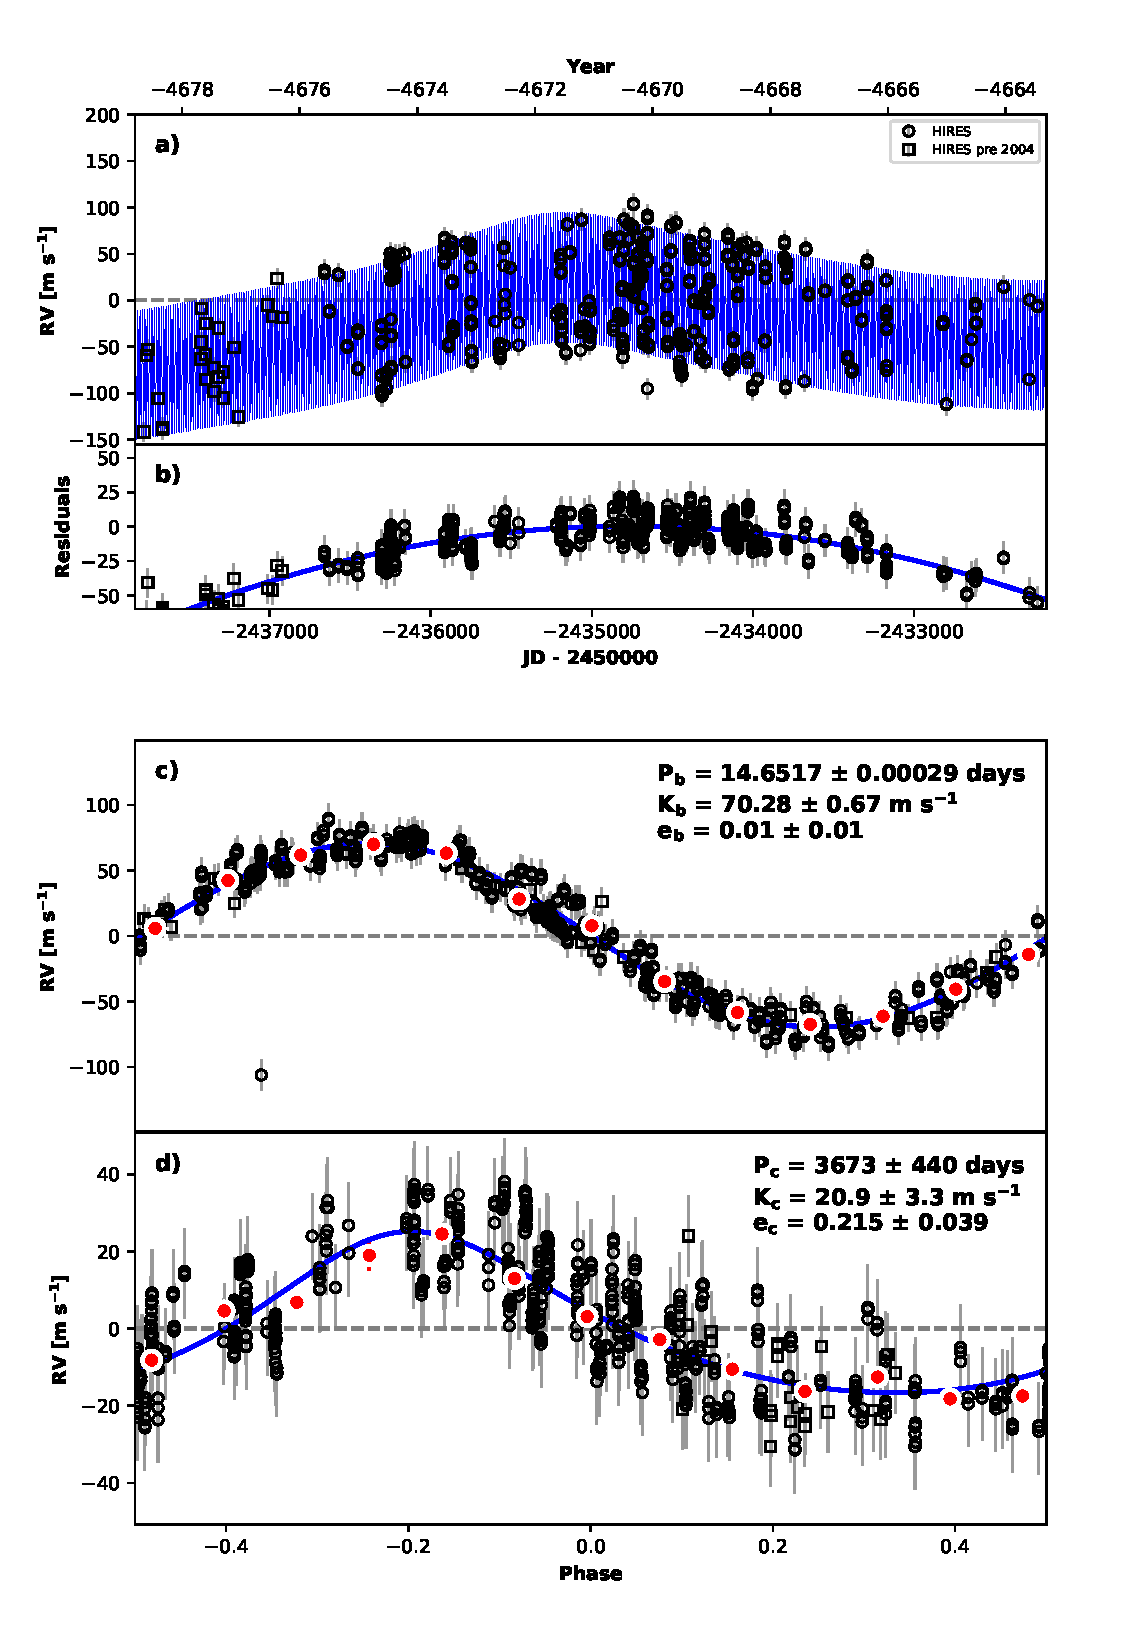
\includegraphics[width=6.5in]{HD75732_2planet_rv_multipanel.pdf}
\caption{
Best-fit 2-planet Keplerian orbital model for HD75732\_2planet.
The maximum likelihood model is plotted while the orbital parameters listed in Table \ref{tab:params}
are the median values of the posterior distributions.
The thin blue line is the best fit 2-planet model. We add in quadrature the RV jitter term(s) listed in Table \ref{tab:params}
with the measurement uncertainties for all RVs.
{\bf b)} Residuals to the best fit 2-planet model.
{\bf c)} RVs phase-folded to the ephemeris of planet b. The Keplerian orbital models for all other planets (if any) have been subtracted.
The small point colors and symbols are the same as in panel {\bf a}.
Red circles (if present) are the same velocities binned in 0.08 units of orbital phase.
The phase-folded model for planet b is shown as the blue line.
Panel {\bf d)} is the same as panel {\bf c)} but for planet HD75732\_2planet c.
}
\end{figure*}

\begin{figure*}[!h]
\centering
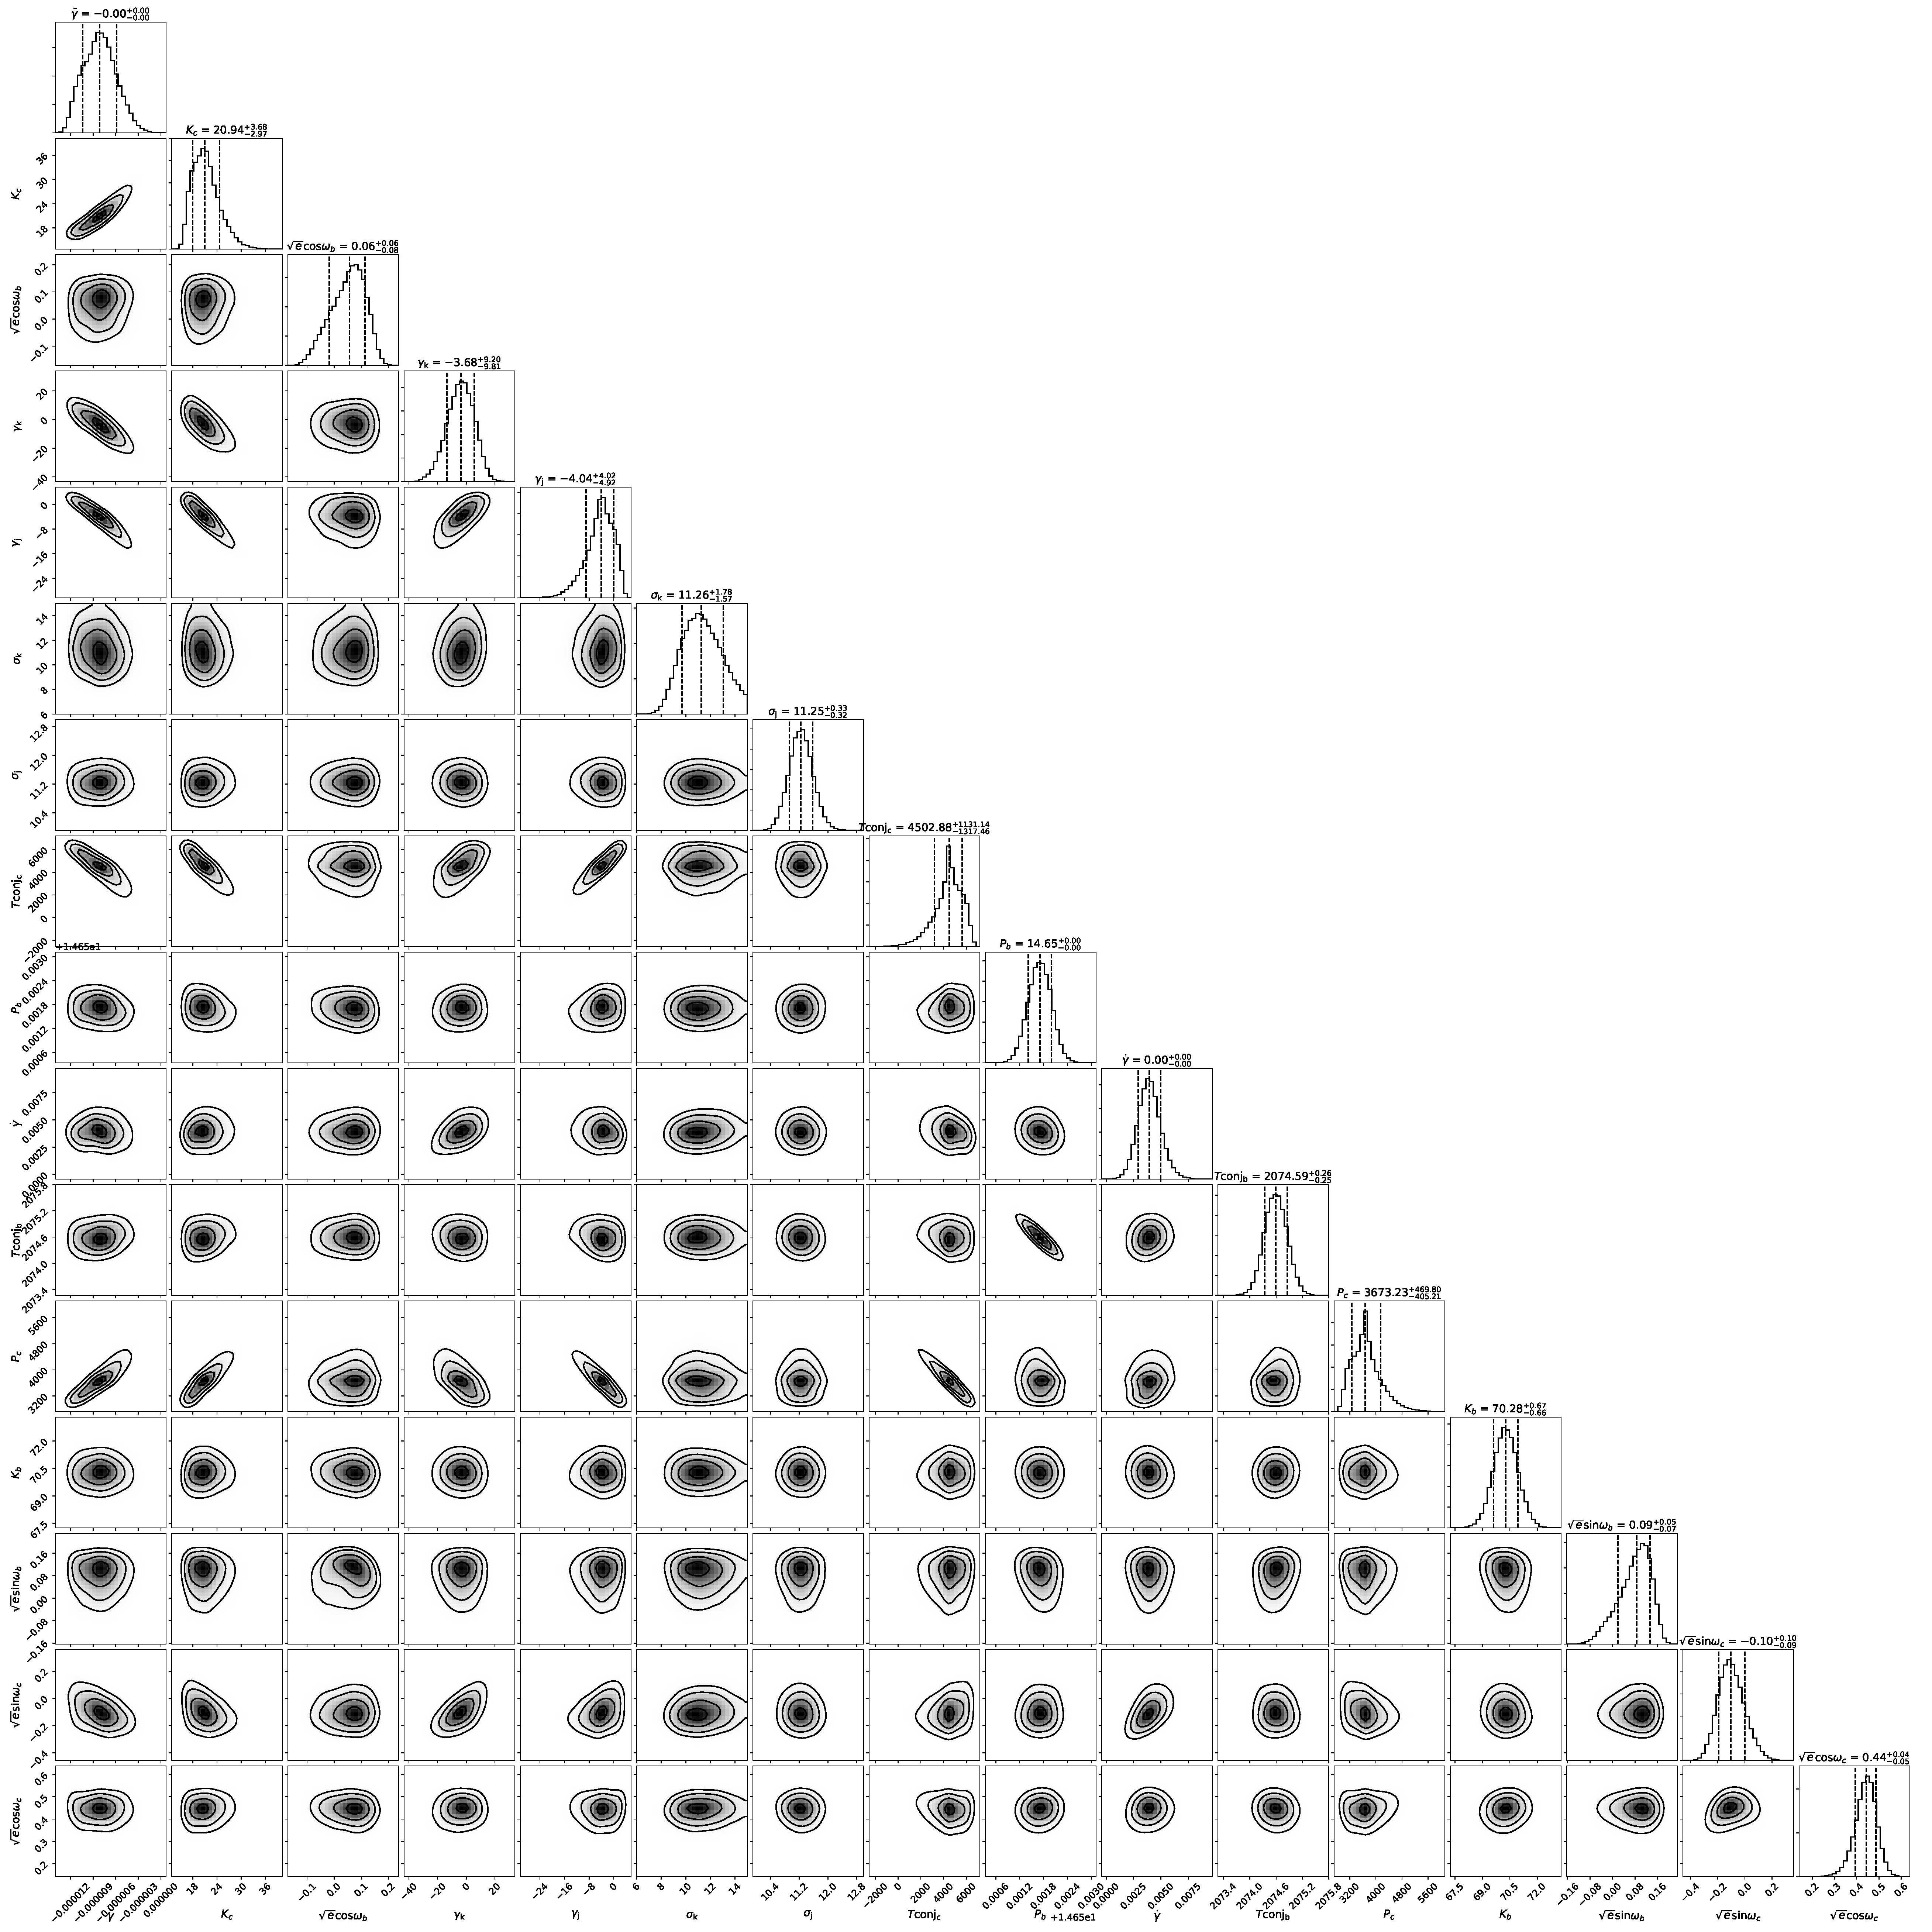
\includegraphics[width=6.5in]{HD75732_2planet_corner.pdf}
\caption{Posterior distributions for all free parameters.}
\end{figure*}

\lfoot{\footnotesize{report produced by \texttt{RadVel} v0.9.2: \href{http://radvel.readthedocs.io}{http://radvel.readthedocs.io}}}
\end{document}